\documentclass[a4paper]{article}
\usepackage[utf8]{inputenc}
\usepackage[slovene]{babel}
\usepackage{graphicx}
\usepackage{hyperref}
\usepackage[nottoc]{tocbibind}
\usepackage{minted}
\usepackage{listings}
\usepackage{caption}
\usepackage{subcaption}
\usepackage{amsmath}
\usepackage{amsfonts}
\usepackage{amssymb}
\usepackage{ dsfont }
\usepackage{siunitx}
\usepackage{multimedia}
\usepackage[table,xcdraw]{xcolor}
\setlength\parindent{0pt}

\definecolor{codegreen}{rgb}{0,0.6,0}
\definecolor{codegray}{rgb}{0.5,0.5,0.5}
\definecolor{codepurple}{rgb}{0.58,0,0.82}
\definecolor{backcolour}{rgb}{0.95,0.95,0.92}
\newcommand{\ddd}{\mathrm{d}}
\newcommand\myworries[1]{\textcolor{red}{#1}}
\newcommand{\Dd}[3][{}]{\frac{\ddd^{#1} #2}{\ddd #3^{#1}}}

\lstdefinestyle{mystyle}{
    backgroundcolor=\color{backcolour},   
    commentstyle=\color{codegreen},
    keywordstyle=\color{magenta},
    numberstyle=\tiny\color{codegray},
    stringstyle=\color{codepurple},
    basicstyle=\ttfamily\footnotesize,
    breakatwhitespace=false,         
    breaklines=true,                 
    captionpos=b,                    
    keepspaces=true,                 
    numbers=left,                    
    numbersep=5pt,                  
    showspaces=false,                
    showstringspaces=false,
    showtabs=false,                  
    tabsize=2
}

\lstset{style=mystyle}

\begin{document}
\begin{titlepage}
    \begin{center}
        
\includegraphics[]{logo.png}
        \vspace*{3cm}
        
        \Huge
        \textbf{Strojno učenje}
        
        \vspace{0.5cm}
        \large
        12. naloga pri Matematično-fizikalnem praktikumu

        \vspace{4.5cm}
        
        \textbf{Avtor:} Marko Urbanč (28191096)\ \\
        \textbf{Predavatelj:} prof. dr. Borut Paul Kerševan\ \\
        
        \vspace{2.8cm}
        
        \large
        8.9.2023
    \end{center}
\end{titlepage}
\tableofcontents
\newpage
\section{Uvod}
Medtem ko se je še nedavno zdelo strojno učenje prava temna magija (vsaj meni), je pravzaprav dandanes
uporaba različnih algoritmov strojnega učenja popolnoma vsakdanja in že rutinska. Ljudje se pravzaprav 
stalno srečujemo z različnimi algoritmi strojnega učenja, ki nam pomagajo pri različnih stvareh, kot so
npr. priporočila na Netflixu, Googlovi iskalni algoritmi, različni algoritmi za prepoznavanje objektov na
slikah, itd. Vse to so algoritmi, ki so zasnovani na strojnem učenju. \\

Prvotno sem želel pustiti prejšnji stavek brez pojasnila, vendar sem se odločil, da bom vseeno napisal nekaj 
besed o kar mislim. Poglejmo prvo Netflix. Netflix je spletna storitev za ogled filmov in serij. Ker je na Netflixu 
ogromno filmov in serij, je težko najti tisto, kar bi si želeli ogledati. Zato Netflix uporablja algoritem, ki na 
podlagi vaših prejšnjih ogledov in ocen priporoča filme in serije, ki bi vam lahko bili všeč 
\cite{lamkhede2021recommendations}. Ampak ne samo to, glede na to iz katere naprave gledate, ob kakšnem času dneva in 
drugih parametrih, ki jim Netflix pravi Kontekst \cite{Steck_Baltrunas_Elahi_Liang_Raimond_Basilico_2021}, pravzaprav 
so pa to \textit{contextual bandits}, ki se uporabljajo v enem okusu strojnega učenja. Več o tem kasneje. V kolikor 
sem uspel razumeti ta članek zgleda, da še več kot to, želijo praktično \textit{in real time} prilagajati priporočila, 
glede na to kakšen je vaš t.i. \textit{intent} \cite{10.1145/2959100.2959174}. Oh in vsi, ki si med seboj delite 
Netflix račune, nikakor ne skrbite, tudi to vas zna nekoč tepst kakšen algoritem strojnega 
učenja \cite{esmaeilzadeh2022abuse}. \\

Nadalje, Google. Google je spletni iskalnik, ki ga praktično vsi uporabljamo. Google uporablja algoritme strojnega
že precej dolgo časa. Leta 2015 so predstavili deep learning sistem RankBrain, ki je bil namenjen izboljšanju
rezultatov iskanja. RankBrain je bil namenjen predvsem iskanju poizvedb, ki jih Google še nikoli ni videl.
RankBrain je bil zasnovan tako, da je na podlagi preteklih iskanj in rezultatov iskanj, ki so jih uporabniki
izbrali, izboljševal rezultate iskanja. Od 2018 naprej so v Google Search v rabi nevronske mreže, ki so namenjene
predvsem izboljšanju rezultatov iskanja. Od 2019 naprej pa Google uporablja tudi BERT \cite{BERT}, ki je bil ogromen
korak naprej v razumevanju naravnega jezika. \\

Na hitro o tipih strojnega učenja oz. osnovnih vrstah algoritmov strojnega učenja. Poznamo

\begin{itemize}
    \item Nadzorovano učenje (supervised learning)
    \begin{itemize}
        \item Klasifikacija (classification): Sortiranje podatkov v razrede. Primer: Razpoznavanje številk na sliki.
        \item Regresija (regression): Modeliranje odvisnosti med podatki. Primer: Napovedovanje cene nepremičnine.
    \end{itemize}
    \item Nenadzorovano učenje (unsupervised learning)
    \item Stimulirano učenje (reinforcement learning)
\end{itemize}

Poglejmo si zdaj uporabo strojnega učenja v fizikalnem kontekstu. V fiziki se strojno učenje uporablja za različne
namene. Največkrat uporabljamo algoritme prvega tipa, torej jih nadzorovano učimo. V fiziki visokih energij se strojno
učenje uporablja za razpoznavanje delcev v detektorjih, za razpoznavanje različnih pojavov, za izboljšanje različnih 
meritev, itd. To je nekaj kar bomo tudi sami počeli v tej nalogi. Iskali bomo Higgsov bozon v podatkih, ki jih je
zbrala ATLAS kolaboracija. \\

\subsection{Kako delujejo algoritmi strojnega učenja?}
Pred tem, pa še osnovno o tem, kako sploh delujejo algoritmi strojnega učenja. Imamo nabor parametrov $\mathcal{D} = 
\{(x_k, y_k)\}_{k=1}^N$, kjer je $x_k = (x_k^1,...x_k^M)$ naključno izbrani vektor z $M$ lastnostmi oz. 
\textit{karakteristikami}, $y_k = (y_k^1,...,y_k^Q)$  pa je vektor $Q$ ciljnih vrednosti, ki so lahko diskretne ali
realna števila ali kaj drugega (npr. barve, ki jim tudi lahko priredimo številske vrednosti). Vrednosti $(x_k, y_k)$
so neodvisne in porazdeljene po neznani porazdelitvi $\mathcal{P}(\cdot,\>\cdot)$. Cilj strojnega učenja je poiskati
oz. priučiti preslikavo $h: \mathbb{R}^Q \rightarrow \mathbb{R}$, ki bo minimizirala pričakovano vrednost funkcije 
izgube (angl. loss function) $\mathcal{L}(h)$

\begin{equation}
    \mathcal{L}(h) = \mathbb{E}\mathrm{L}(\vec{y}, \vec{h}(\vec{x})) = \frac{1}{N} \sum_{k=1}^N{\mathrm{L}(y_k, \vec{h}(x_k))}\>,
\end{equation}

kjer je $\mathrm{L}(\cdot,\cdot)$ gladka funkcija, ki opisuje oceno za kvaliteto napovedi, pri čemer so $(\vec{x}, \vec{y})$
neodvisno vzorčene iz nabora $\mathcal{D}$ po porazdelitvi $\mathcal{P}(\cdot,\cdot)$. Po koncu učenja imamo torej na voljo 
funkcijo $h(\vec{x})$, ki nam za nek vhodni nabor vrednosti $\hat{x}$ poda napoved $\hat{y} = \vec{h}(\hat{x})$., ki ustrezno
kategorizira ta nabor vrednosti.\\

Funkcije $\vec{h}$ so v praksi sestavljene iz množice preprostih funkcij z prostimi parametri, kar na koncu seveda pomeni 
velik skupni nabor neznanih parametrov in zahteven postopek postopek minimizacije funkcije izgube.

\subsection{Odločitvena drevesa (Decision trees)}
Odločitvena drevesa so ena izmed najbolj preprostih metod strojnega učenja. Odločitvena drevesa so sestavljena iz
vozlišč in povezav. Vozlišča so povezana z povezavami, ki so lahko usmerjene ali neusmerjene. Osnovni gradnik
odločitvenega drevesa je kar stopničasta funkcija $\mathrm{H}(x_i,-t_i) = 0,1$, ki je enaka ena za $x_i > t_i$ in
nič za $x_i < t_i$, kjer je $x_i$ ena izmed karakteristik in $t_i$ neznani parameter. Iz skupine takšnih funkcij,
ki predstavljajo binarne odločitve lahko skonstruiramo končno uteženo funkcijo 

\begin{equation}
    \vec{h} = \sum_{i=1}^J{\vec{w}_i \mathrm{H}(x_i, -t_i)}\>,
\end{equation}

kjer so $\vec{w}_i$ vektorji neznanih uteži. Tako $t_i$ kot $\vec{w}_i$ lahko določimo, v procesu učenja. 
Nadgradnjo odločitvenih dreves predstavljajo pospešena odločitvena drevesa (angl. boosted decision trees), ki uporabljajo
več odločitvenih dreves, ki so med seboj povezana. Temeljijo pa na Gradient Boosting algoritmu \cite{Friedman_2001}, ki je 
bil razvit leta 1999 in je bil namenjen izboljšanju napovedi. Gradient Boosting algoritem je bil razvit za regresijske 
probleme, vendar se ga da uporabiti tudi za klasifikacijske probleme in je v praksi zelo uspešen. \\

\subsection{Nevronske mreže (Neural networks)}
Pri nevronskih mrežah gre za to, da imamo množico nevronov, ki so med seboj povezani. Vsak nevron je povezan z vsakim 
nevronom v naslednjem sloju. Nevroni so med seboj povezani z utežmi, ki jih lahko spreminjamo. Slojev je lahko več,
odvisno od tega, kako kompleksen model želimo. Poznamo vidne sloje, skrite sloje in izhodne sloje. Nevroni v vidnem
sloju so povezani z vhodnimi podatki, nevroni v skritih slojih so žal za nas neke sorte \textit{black box}, ki ga
ne moremo razumeti, izhodni sloj pa nam poda napoved. Nevronske mreže so zelo uspešne pri klasifikaciji in regresiji. 
Obstaja tudi cel kup podvrst nevronskih mrež, kot so npr. konvolucijske nevronske mreže, ki so zelo uspešne pri
razpoznavanju objektov na slikah, rekurentne nevronske mreže, ki so zelo uspešne pri razpoznavanju govora, itd.\\

Osnoven gradnik nevronskih mrež je \textit{perceptron}, ki ga opisuje funkcija 

\begin{equation}
    \mathrm{h}_{w,b} = \theta(\vec{w}^\intercal\cdot \vec{X}+ b)\>,
\end{equation}

kjer je $\vec{w}$ vektor uteži, $\vec{X}$ vektor vhodnih vrednosti, $b$ pa je neka konstanta, ki ji pravimo \textit{bias}.
Preko tega tvorimo uteženo vsoto. Funkcije $\theta$ se imenuje \textit{aktivacijska funkcija}. Najbolj pogosta je
\textit{sigmoidna} funkcija, ki je definirana kot

\begin{equation}
    \theta(x) = \frac{1}{1+e^{-x}}\>.
\end{equation}

Ta vpelje neke vrste nelinearnost v model. Če bi uporabili linearno funkcijo, bi namreč dobili linearno preslikavo. 
Dandanes se sicer poleg sigmoidne funkcije uporabljajo tudi druge funkcije, verjetno je najbolj znana \textit{ReLU}
funkcija \cite{agarap2019deep}, ki je definirana kot

\begin{equation}
    \theta(x) = \max(0,x)\>.
\end{equation}

Ta je boljša zaradi več razlogov, ampak v glavnem so prednosti, da se jo bistveno hitreje računa in da je bolj odporna
na \textit{vanishing gradient} problem. Nevronske mreže se učijo preko dveh ključnih algoritmov in sicer \textit{back propagation}
in \textit{gradient descent}. Back propagation je algoritem, ki nam omogoča, da izračunamo gradient funkcije izgube po
vseh utežeh v nevronski mreži. S tem lahko popravimo uteži v nevronski mreži za en korak. Gradient descent pa je algoritem,
ki nam omogoča, da se sprehodimo po funkciji izgube in poiščemo lokalni minimum. Problem, ki ga ima recimo sigmoida je, da
ima majhno vrednost gradienta, drugod pa se funkcija asimptotsko obnaša in je gradient tam enak nič. Kar se zgodi je, da 
se zniža vrednost gradienta za vsak sloj, ki ga imamo v nevronski mreži. To pomeni, da se bodo prvi sloji nepravilno 
učili. Rečeno malo drugače, njihov gradient izgine in ker se to zgodi, bo tudi aktivacijska funkcija premikala vrednost 
proti nič. Z uporabo ReLU funkcije tega problema nimamo, saj je gradient konstanten in ne izgine. To pomeni, da nam modeli 
v splošnem hitreje konvergirajo. Seveda pa tudi ReLU funkcija ni brez svojih napak. Pojavi se lahko ravno kontra pojav, 
torej \textit{exploding gradient}. Obstaja potem cela vrsta izboljšav, da bi se temu izognili. \\

Nevronska mreža je sestavljena iz poljubne topologije prej omenjenih perceptronov, ki na začetku sprejmejo karakteristiko 
dogodka $\vec{x}$ v končni fazi pa vrnejo napoved $\hat{y}$, ki mora biti lim bližje pravi vrednosti $y$. Z uporabo ustrezne
funkcije izgube, recimo MSE, definiran kot

\begin{equation}
    \mathrm{MSE} = \mathcal{L}(h) = \mathbb{E}||\vec{y}-\hat{y}||^2\>,
\end{equation}

se problem znova prevede na minimizacijo, kjer znova iščemo minimum funkcije izgube, za neznan nabor uteži $\vec{w}$ in konstant 
$b_i$. Globoke nevronske mreže niso nič drugega, kot velike nevronske mreže, ali skupine le-teh.
\section{Naloga}
Naloga nam tokrat poda ves material potreben, tako kodo, kot vzorce, za ločevanje dogodkov Higgsovega bozona od ostalih procesov
ozadja. V naboru simuliranih dogodkov je 18 karakteristik, katerih vsaka posamezno zelo slabo loči signal od ozadja. Preko ML pa 
lahko dosežemo kar dober uspeh.\\

Naloga zahteva od nas da za obe metodi, tako BDT kot NN, določimo uspešnost in narišemo ROC krivuljo, za nekaj tipičnih konfiguracij.
Naj bomo pozorni na vpliv vhodnih parametrov na uspešnost in na število uporabljenih spremenljivk.

\section{Opis reševanja}
Reševanja sem se lotil tako, da sem si najprej malo ogledal profesorjevo kodo. Kmalu sem ugotovil, da despite 
komentarjem in kakšnega docstringa v kodi, bo za razumevanje šlo hitreje če si sam napišem programe. As usual 
je Python standardno orodje z bibliotekami \texttt{numpy}, \texttt{pandas}, \texttt{matplotlib}, \texttt{scikit-learn},
\texttt{catboost} in \texttt{torch}. Sparking the debate oz. tekmovalnost med \texttt{tensorflow}, ki ga je uporabil 
profesor in \texttt{pytorch}, ki ga imam jaz raje. \\

Kot je zdaj navada sem si napisal nekaj razredov za lažje delo. Začel sem z razredom za BDT modele, ki sem ga poimenoval
\texttt{BoostMe}. V njem sem definiral metode za učenje modela, za napovedovanje in za izris ROC krivulje. Za učenje sem
uporabljal \texttt{catboost} knjižnico, bolj specifično \texttt{CatBoostClassifier}. Se mi zdi, da sem kar navdušen nad
njo. \\

Nato sem napisal razred za NN modele, ki sem ga poimenoval \texttt{WhereArtThouHiggs}. V njem sem definiral metode za
ustvarjenje modela, za učenje modela, za napovedovanje in za izris ROC krivulje. Za ustvarjanje modela sem uporabil
\texttt{torch} knjižnico, bolj specifično \texttt{torch.nn.Sequential}, ki sem ga napolnil z tremi sloji 
\texttt{torch.nn.Linear} in aktivacijsko funkcijo \texttt{torch.nn.ReLU}. Zadnji sloj ima Sigmoidno aktivacijsko funkcijo.
\texttt{torch.nn.Sigmoid}. Za učenje sem uporabil \textbf{Stochastic gradient descent} \texttt{torch.optim.SGD} in kot smo 
rekli v uvodu kar \texttt{torch.nn.MSELoss} za funkcijo izgube.
\section{Rezultati}
\subsection{BDT}
Glavni parameter, ki ga lahko spreminjamo pri algoritmu BDT je število dreves, ki jih uporabimo. Začel sem z 100 drevesi in
nato število dreves povečeval. Logično sledi obvezna primerjava med časom izračunov na GPU in na CPU. GPU je RTX 3060Ti,
CPU pa Ryzen 5 3600X. Rezultati so prikazani na sliki \ref{fig:BDT_times}. \\

\begin{figure}[H]
    \centering
    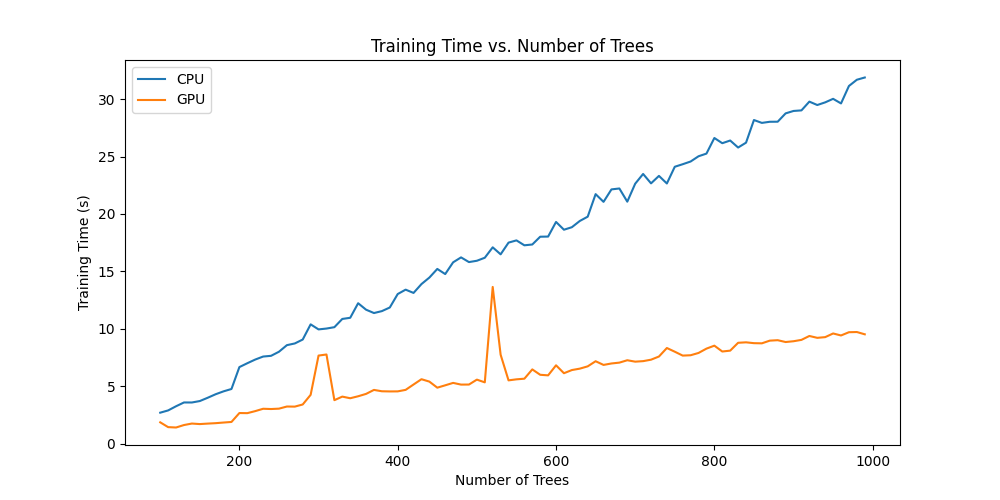
\includegraphics[width=0.8\textwidth]{../images/raw_performance.png}
    \caption{Čas izračuna BDT modela na GPU in CPU.}
    \label{fig:BDT_times}
\end{figure}

Kot vidimo je čas izračuna na GPU veliko hitrejši. Čeprav je to pričakovano, je vseeno zanimivo videti, da je razlika v času
izračuna kar precejšnja. Zdaj lahko vsi prepričujemo svoje starše, da potrebujemo grafično kartico za študij. Smiselno je pogledati
še druga dva pomembna parametra in sicer \textit{learning rate} in \textit{max\_depth}. So na sliki \ref{fig:BDT_params}. \\

\begin{figure}[H]
    \centering
    \makebox[\textwidth][c]{%
    \begin{minipage}{0.70\textwidth}
        \centering
        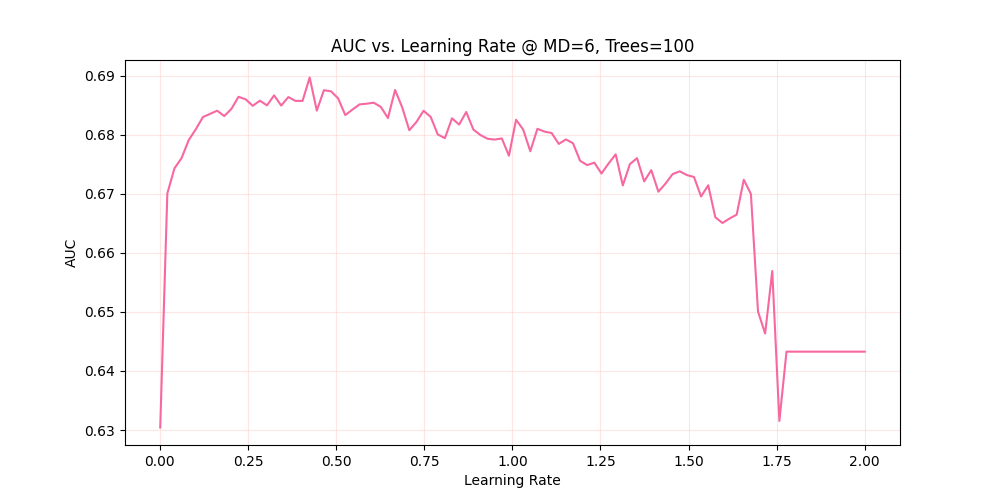
\includegraphics[width=\linewidth]{../images/lr_sweepv2.png}
    \end{minipage}%
    \hspace{0.1\textwidth}% 
    \begin{minipage}{0.70\textwidth}
        \centering
        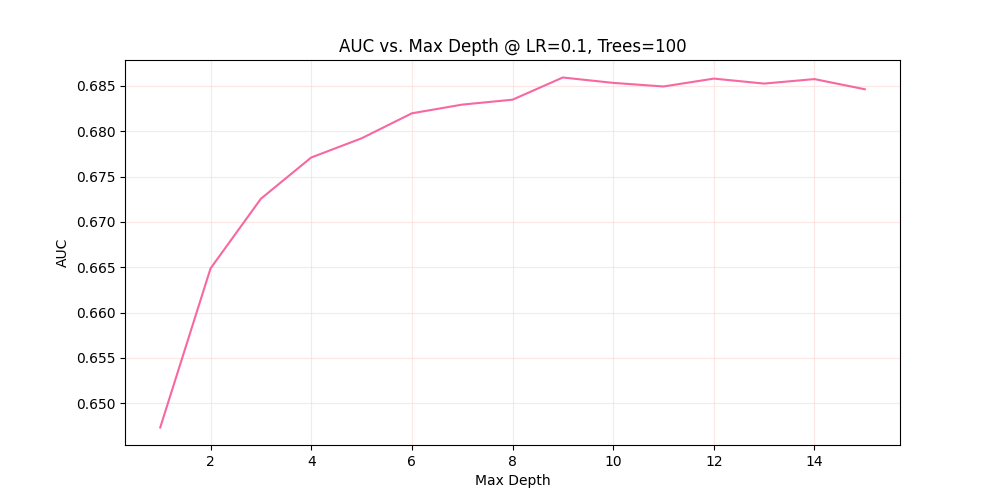
\includegraphics[width=\linewidth]{../images/md_sweep.png}
    \end{minipage}%
    }
    \caption{Vpliv \textit{learning rate} in \textit{max\_depth} na uspešnost BDT modela.}
    \label{fig:BDT_params}
\end{figure}

Vidimo, da ocena za uspešnost modela lepo narašča z večanjem \textit{max\_depth} in \textit{learning rate}. Očitno v temu 
primeru so vse globine od $6$ naprej odveč ker je rezultat relativno konstanten. \textit{Learning rate} ima velik vpliv 
na uspešnost modela in vidimo da je lepo izbrati neko srednjo vrednost. Premala vrednost in bo model počasen, prevelika
vrednost in bo model neuspešen. Izrisal sem pa tudi kako se vrednost funkcije izgube manjša za model z $100$ drevesi, 
\textit{max\_depth} $= 6$ in \textit{learning rate} $= 0.1$. Rezultat je na sliki \ref{fig:BDT_ROC}. \\

\begin{figure}[H]
    \centering
    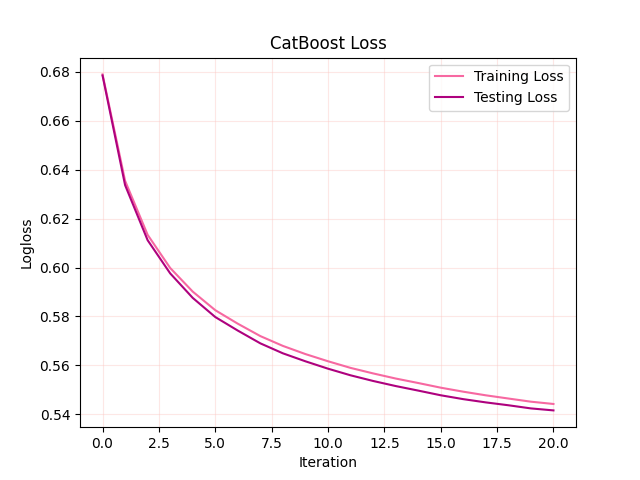
\includegraphics[width=0.8\textwidth]{../images/catboost_loss.png}
    \caption{ROC krivulja za BDT model z $100$ drevesi, \textit{max\_depth} $= 6$ in \textit{learning rate} $= 0.1$.}
    \label{fig:BDT_ROC}
\end{figure}

In seveda tudi ROC krivuljo za model z prej omenjenemi parametri in za model, ki ima spremenjeno število dreves na $1000$. 
Rezultat je na sliki \ref{fig:BDT_ROC}. \\

\begin{figure}[H]
    \centering
    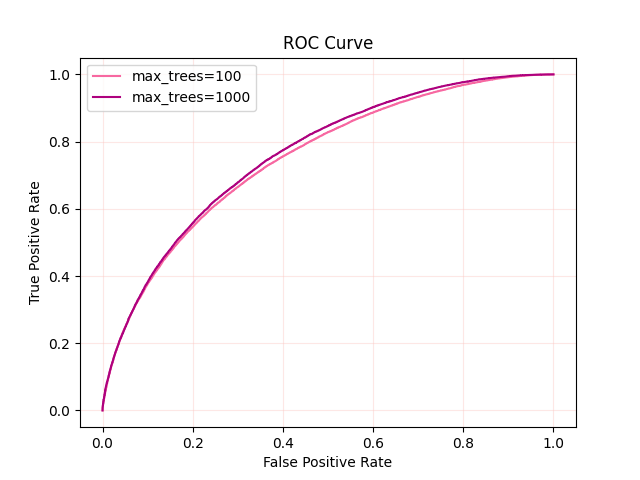
\includegraphics[width=0.8\textwidth]{../images/catboost_roc.png}
    \caption{ROC krivulja za BDT model z $100$ drevesi, \textit{max\_depth} $= 6$ in \textit{learning rate} $= 0.1$ ter za 
    model z $1000$ drevesi, \textit{max\_depth} $= 6$ in \textit{learning rate} $= 0.1$.}
    \label{fig:BDT_ROC}
\end{figure}

Vidimo, da je razlika med njima pravzaprav precej marginalna. Glede na to, da je prvi model porabil le $1.57$ s za učenje,
medtem ko je drugi porabil $10.45$ s, se mi zdi da je prvi model boljša izbira, glede na majhno razliko v uspešnosti, a relativno 
veliko ceno v času izračuna.
\subsection{NN}
V glavnem sem tu poskusil rekreirati profesorjeve rezultate. Zaradi velikosti podatkovnega seta in pa narave 
učenja NN modelov, traja učenje kar nekaj časa. Žal zaradi mojih lastnih napak, nimam dovolj časa, da bi se 
igral z vsemi parametri in bi lahko naredil kakšno boljšo analizo. 

\section{Komentarji in izboljšave}


\newpage
\bibliographystyle{unsrt}
\bibliography{sources}
\end{document}
